\chapter{Introduction}

The motivation for this project lies within the roots of amateur radio. Amateur radio operators, commonly referred to as hams, are a community of people who are joined together by their enjoyment for hearing themselves talk and through coming up with creative solutions to their communication problems. The Automatic Packet Reporting System (APRS) is one example of a creative communication solution that the community utilizes.

APRS is a digital communication method commonly used by hams in order to report their GPS location in order to facilitate local area awareness to fellow operators. However, it has many more uses than just GPS tracking. A lot of the infrastructure for this system is based on retired commercial hardware that could be purchased at a low cost. The Bell 202 modem was patented in 1984 and the FSK modulation scheme used to transmit the data was approved by the International Telecommunication Union in 1988 [1, 2]. However, the actual specification for APRS was published in 2000, 12 years after these technologies were finalized [3].

This timeline helps to reinforce the fact that the technologies used for this system are old and far from cutting edge. Recently, in 2012, Sivan Toledo put together a Java based software package for demodulating these Bell 202, specifically APRS, packets. Using this package as the framework for testing other demodulation algorithms more insight was gained into software demodulation. Software demodulation provides a low cost alternative to hardware demodulators since users can run the software on hardware that they already possess. For example APRSDroid (an app in the Google’s Android Play Store) directly imports JavaAX25’s software demodulation [5]. 

\begin{figure}
  \centering
  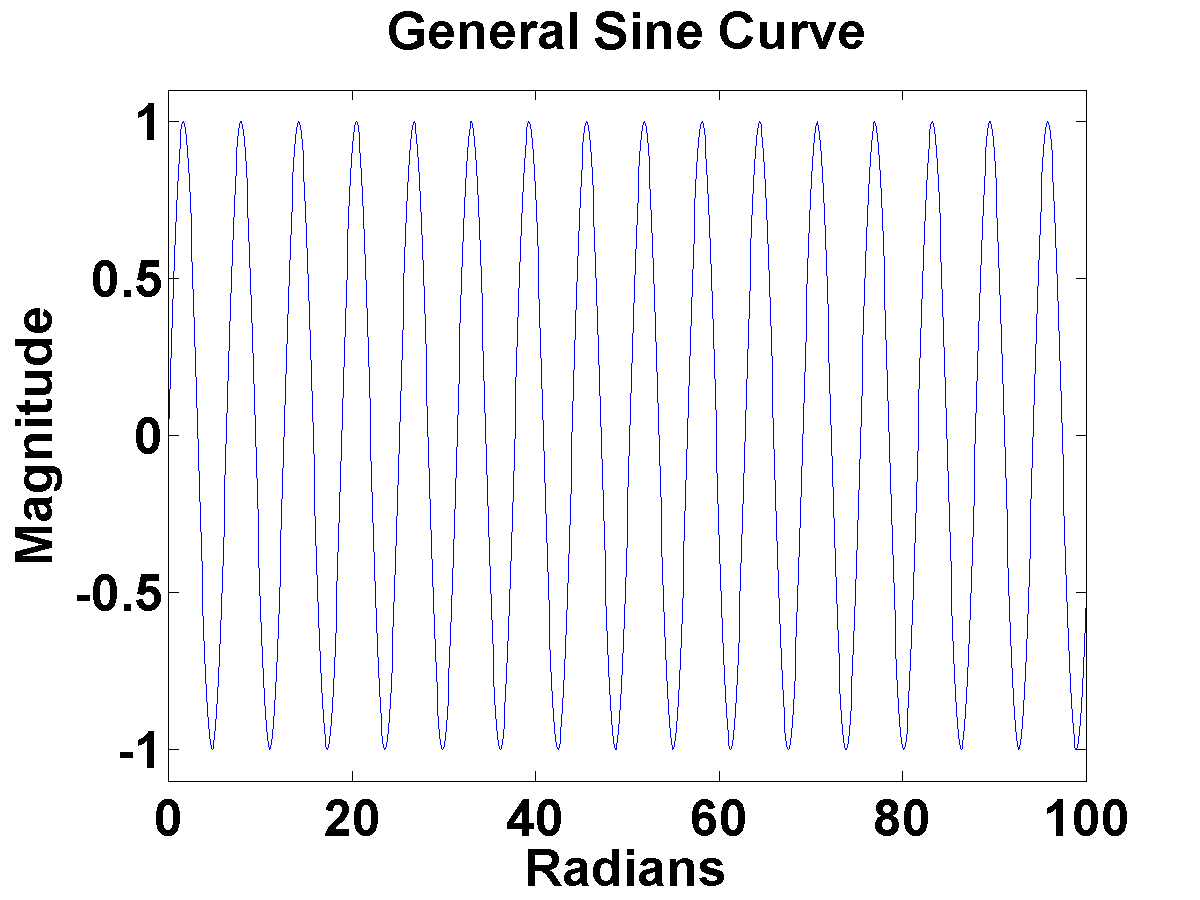
\includegraphics[width=0.75\linewidth]{images/GeneralSineCurve.png}
%  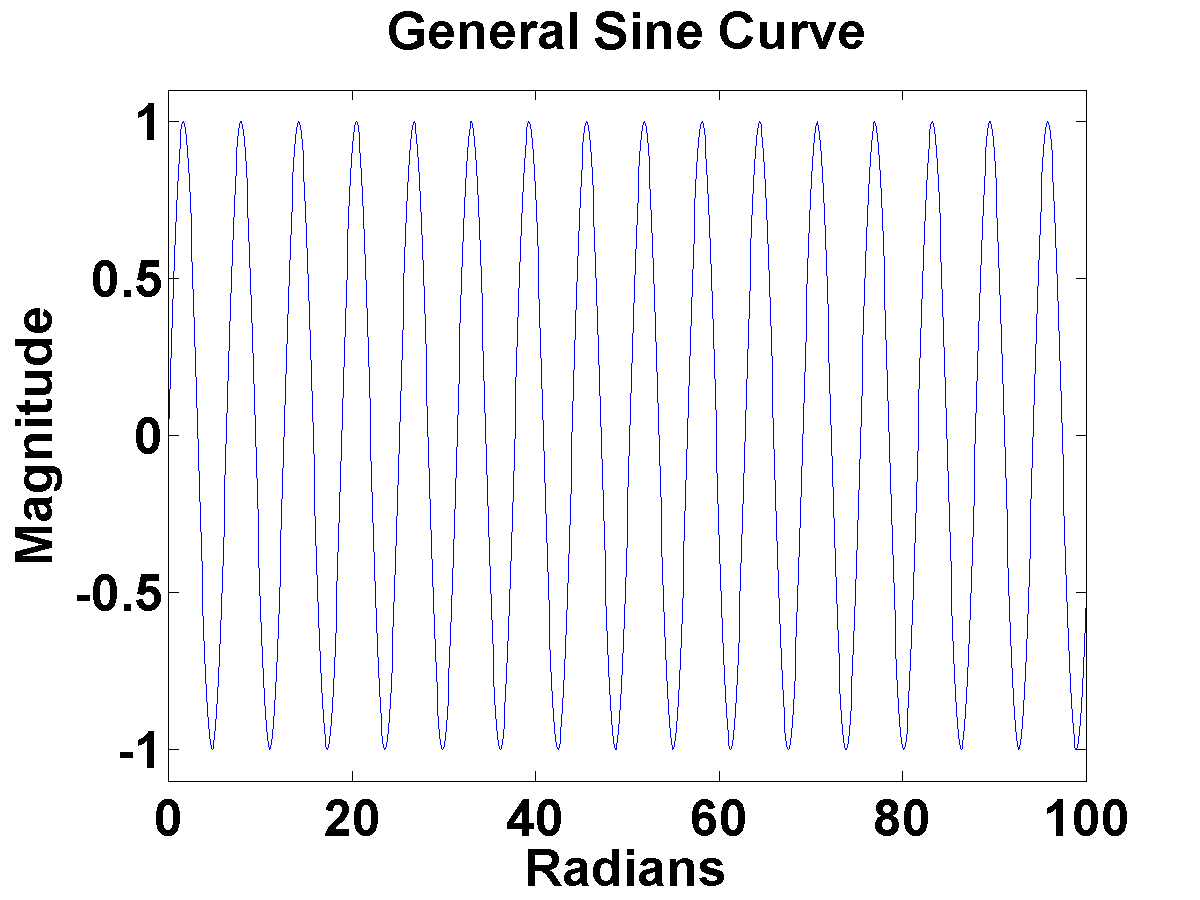
\includegraphics{images/GeneralSineCurve.png}
  \caption{Example Bell202 signal for the bit stream 010101}
\end{figure}

As mentioned thus far, software provides a viable low cost alternative to dedicated hardware, but still has some weaknesses that need to be addressed to improve reliability to match hardware. Section 2 goes into background information. Section 3 gives a summary and detailed information on Toledo's JavaAX25 package. Section 4 goes into our implementation specifics, discussing our different algorithms and interesting edge cases that we encountered. Section 5 describes the methods for testing the implementations. Section 6 discusses results including decoded packets and some rough memory usage analysis. Section 7 comments on areas for future work, and finally section 8 concludes this research project.
